\documentclass[a4paper]{article}

\usepackage[T2A]{fontenc}
\usepackage[russian]{babel}
\usepackage{graphicx}
\usepackage{float}
\usepackage{hyperref}
\usepackage{amsmath, amssymb}
\usepackage{caption}
\usepackage{geometry}
\usepackage{pdfpages}
\usepackage{indentfirst}
\usepackage{gensymb}
\usepackage{lipsum}
\usepackage{relsize}
\usepackage{amsmath}
\geometry{top=2cm,bottom=2cm,left=2cm,right=2cm}

\newcommand{\minus}{\scalebox{0.75}[1.0]{$-$}}

\linespread{1.25}

\begin{document}

\begin{center}
\textsc{ИТМО\\[3mm]
Физический факультет} \\[3mm]

\end{center}
\vspace{5mm}

\vspace{2mm}
\line(1,0){\textwidth}
\vspace{5mm}
\begin{minipage}{0.4\textwidth}
    Группа: Z3144 \\
    Студент: Григорий Горбушкин\\
    \vspace{1mm}
\end{minipage}
\hfill
\vspace{1mm}
\line(1,0){\textwidth}



\section{ \textbf{Цели работы}}

 Экспериментальное измерение удельной теплоёмкости мате
риала образца.

\section{\textbf{Задачи}}

Получить зависимость увеличения температуры образцов с течением времени при нагревании.



\section{\textbf{Теоретическое введение}}

 Теплоёмкостью называется величина, равная отношению бесконечно малого количества теплоты $\delta Q$, полученного телом при нагревании, к приращению его температуры $d T$ :


\begin{equation*}
C=\frac{\delta Q}{d T} \tag{1}
\end{equation*}


Теплоёмкость, отнесённая к единице массы вещества, называется удельной теплоёмкостью:


\begin{equation*}
c=\frac{C}{m}=\frac{1}{m} \frac{\delta Q}{d T} \tag{2}
\end{equation*}


В данной лабораторной работе производится нагревание исследуемого образца в тепловой камере. Обозначим теплоёмкость образца через $C$, а теплоёмкость камеры - через $C_{0}$. Мощность нагревателя определяется как произведение измеряемых в ходе эксперимента силы тока и напряжения в его цепи:


\begin{equation*}
P=I U . \tag{3}
\end{equation*}


Часть энергии, выделяемой нагревателем за интервал времени $d t$, расходуется на увеличение температуры образца и тепловой камеры на $d T$, часть уходит в окружающую среду через её стенки:


\begin{equation*}
\left(C+C_{0}\right) d T=P d t-K\left(T-T_{\text {окр }}\right) d t . \tag{4}
\end{equation*}


Здесь $T$ - температура образца, $T_{\text {окр }}$ - температура воздуха вокруг камеры, которая поддерживается постоянной в ходе всего эксперимента. Коэффициент $K$ в этой формуле определяется только параметрами установки и разностью температур рабочего объёма камеры и воздуха вокруг неё. Поскольку в ходе эксперимента относительное изменение температуры образца не очень велико, последней зависимостью можно пренебречь и считать коэффициент $K$ неизменным на протяжении всего эксперимента. Решаем уравнение (4), чтобы получить зависимость температуры образца от времени нагревания:


\begin{equation*}
\frac{\left(C+C_{0}\right) d T}{P-K\left(T-T_{\text {окр }}\right)}=d t \tag{5}
\end{equation*}


Для того, чтобы решить уравнение, перейдём к новой переменной:


\begin{equation*}
Z=P-K\left(T-T_{\text {окр }}\right), d Z=-K d T . \tag{6}
\end{equation*}


Формула (5) с новой переменной приобретает вид:


\begin{equation*}
\frac{\left(C+C_{0}\right) d Z}{K Z}=-d t \tag{7}
\end{equation*}


После интегрирования и подстановки выражения (6) для $Z$ получим:


\begin{equation*}
\ln \left(P-K\left(T-T_{\text {окр }}\right)\right)=-\frac{K t}{C+C_{0}}+\text { const } . \tag{8}
\end{equation*}


Постоянную в этом уравнении определяем из условия, что в момент начала отсчёта времени $t=0$ температура рабочего объёма камеры была равна температуре окружающей среды $T_{\text {окр }}$, т.е. const $=\ln (P)$. С учетом этого после потенцирования уравнения $(8)$ получаем:


\begin{equation*}
P-K\left(T-T_{\text {окр }}\right)=P \exp \left(-\frac{K t}{C+C_{0}}\right) . \tag{9}
\end{equation*}


Отсюда зависимость температуры камеры от времени для процесса нагревания камеры с образцом имеет вид:


\begin{equation*}
T-T_{\text {окр }}=\frac{P}{K}\left(1-\exp \left(-\frac{K}{C_{0}+C} t\right)\right) . \tag{10}
\end{equation*}


Аналогично для нагревания пустой камеры находим:


\begin{equation*}
T-T_{\text {окр }}=\frac{P}{K}\left(1-\exp \left(-\frac{K}{C_{0}} t\right)\right) . \tag{11}
\end{equation*}


Продифференцируем уравнения (10) и (11) по времени и прологарифмируем получившиеся уравнения. Для нагревания камеры с образцом получим:


\begin{equation*}
\ln \left(\frac{d\left(T-T_{\text {окр }}\right)}{d t}\right)=\ln \frac{P}{C_{0}+C}-\frac{K}{C_{0}+C} t, \tag{12}
\end{equation*}


а для нагревания пустой камеры:


\begin{equation*}
\ln \left(\frac{d\left(T-T_{\text {окр }}\right)}{d t}\right)=\ln \frac{P}{C_{0}}-\frac{K}{C_{0}} t . \tag{13}
\end{equation*}


Для того чтобы найти теплоемкость образца, необходимо дважды провести измерения: в первом случае - нагревать пустую камеру, во втором случае - камеру с образцом. По результатам этих измерений необходимо построить графики зависимости от времени выражений, стоящих в левых частях уравнений (12) и (13). Зная мощность нагревателя, по свободным коэффициентам этих графиков можно будет определить теплоемкость камеры с образцом $C+C_{0}$, теплоёмкость самой камеры $C_{0}$ и по разности этих теплоемкостей найти теплоёмкость образца. По известным теплоемкости $C$ и массе $m$ образца по формуле (2) можно вычислить удельную теплоёмкость материала образца. Масса образца измеряется в работе с помощью лабораторных весов. Дополнительна проверка теории, приводящей к формулам (12) и (13) состоит в следующем. Отношение теплоемкостей $\frac{C_{0}+C}{C_{0}}$ можно оценить по частному угловых коэффициентов в этих формулах и сравнить с соответствующим результатом, полученным из анализа свободных коэффициентов. Хорошее совпадение результатов подтвердит, что предложенная теория применима к данному эксперименту.

\section{\textbf{Экспериментальная установка}}

\begin{figure}[H]
\begin{center}
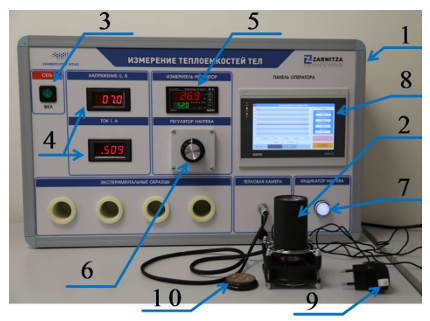
\includegraphics[width=0.6\textwidth]{2}
\end{center}
\end{figure}
\begin{enumerate} 
  \item Моноблок ”Измерение теплоёмкости тел” с набором функци
ональных модулей;
  \item Тепловая камера, в которой осуществляется нагрев образцов;
  \item Кнопка включение питания моноблока;
  \item Индикаторы значений напряжения и тока нагревательного элемента тепловой камеры;
  \item Индикаторы значений текущей температуры (красный) и предельной температуры (зеленый);
  \item Ручка регулятора напряжения, подаваемого на нагревательный элемент;
  \item Индикатор подачи напряжения на нагревательный элемент;
  \item Графический сенсорный дисплей для отображения графика тем
пературы и контроля управления стендом;
  \item Блок питания вентилятора, закрепленного под камерой (тум
блер включения расположен на блоке питания);
  \item Съёмная крышка тепловой камеры.
\end{enumerate}



\section{\textbf{Данные}}
\begin{figure}[H]
\begin{center}
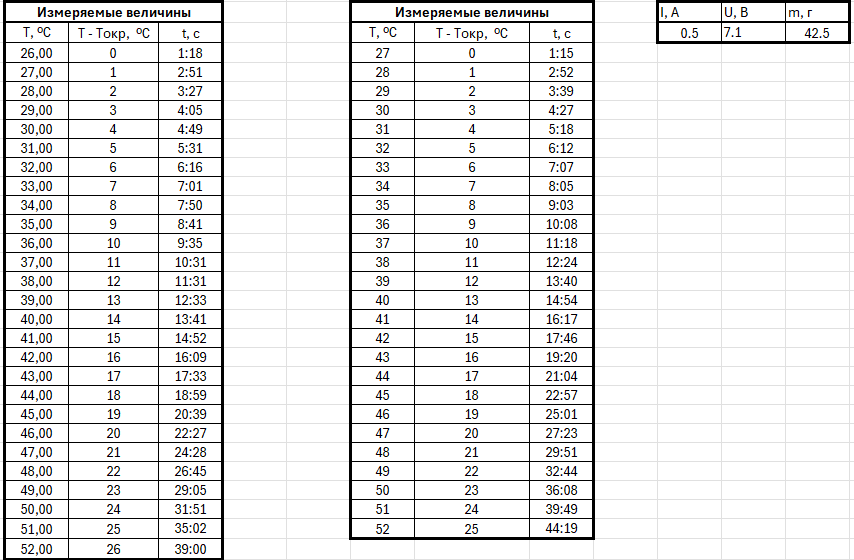
\includegraphics[width=0.6\textwidth]{1}
\end{center}
\end{figure}


\section{\textbf{Обработка результатов}}

Для нахождения численного хначения производной, воспользуемся формулой (14).
\begin{equation*}
\dfrac{d(T-T_{окр})}{dt} \approx \dfrac{2\degree C}{t_{i+1}-t_{i-1}}. \tag{14}
\end{equation*}



В python строим графики зависимости $\dfrac{d(T-T_{окр})}{dt}$ от $t$.
\begin{figure}[H]
\begin{center}
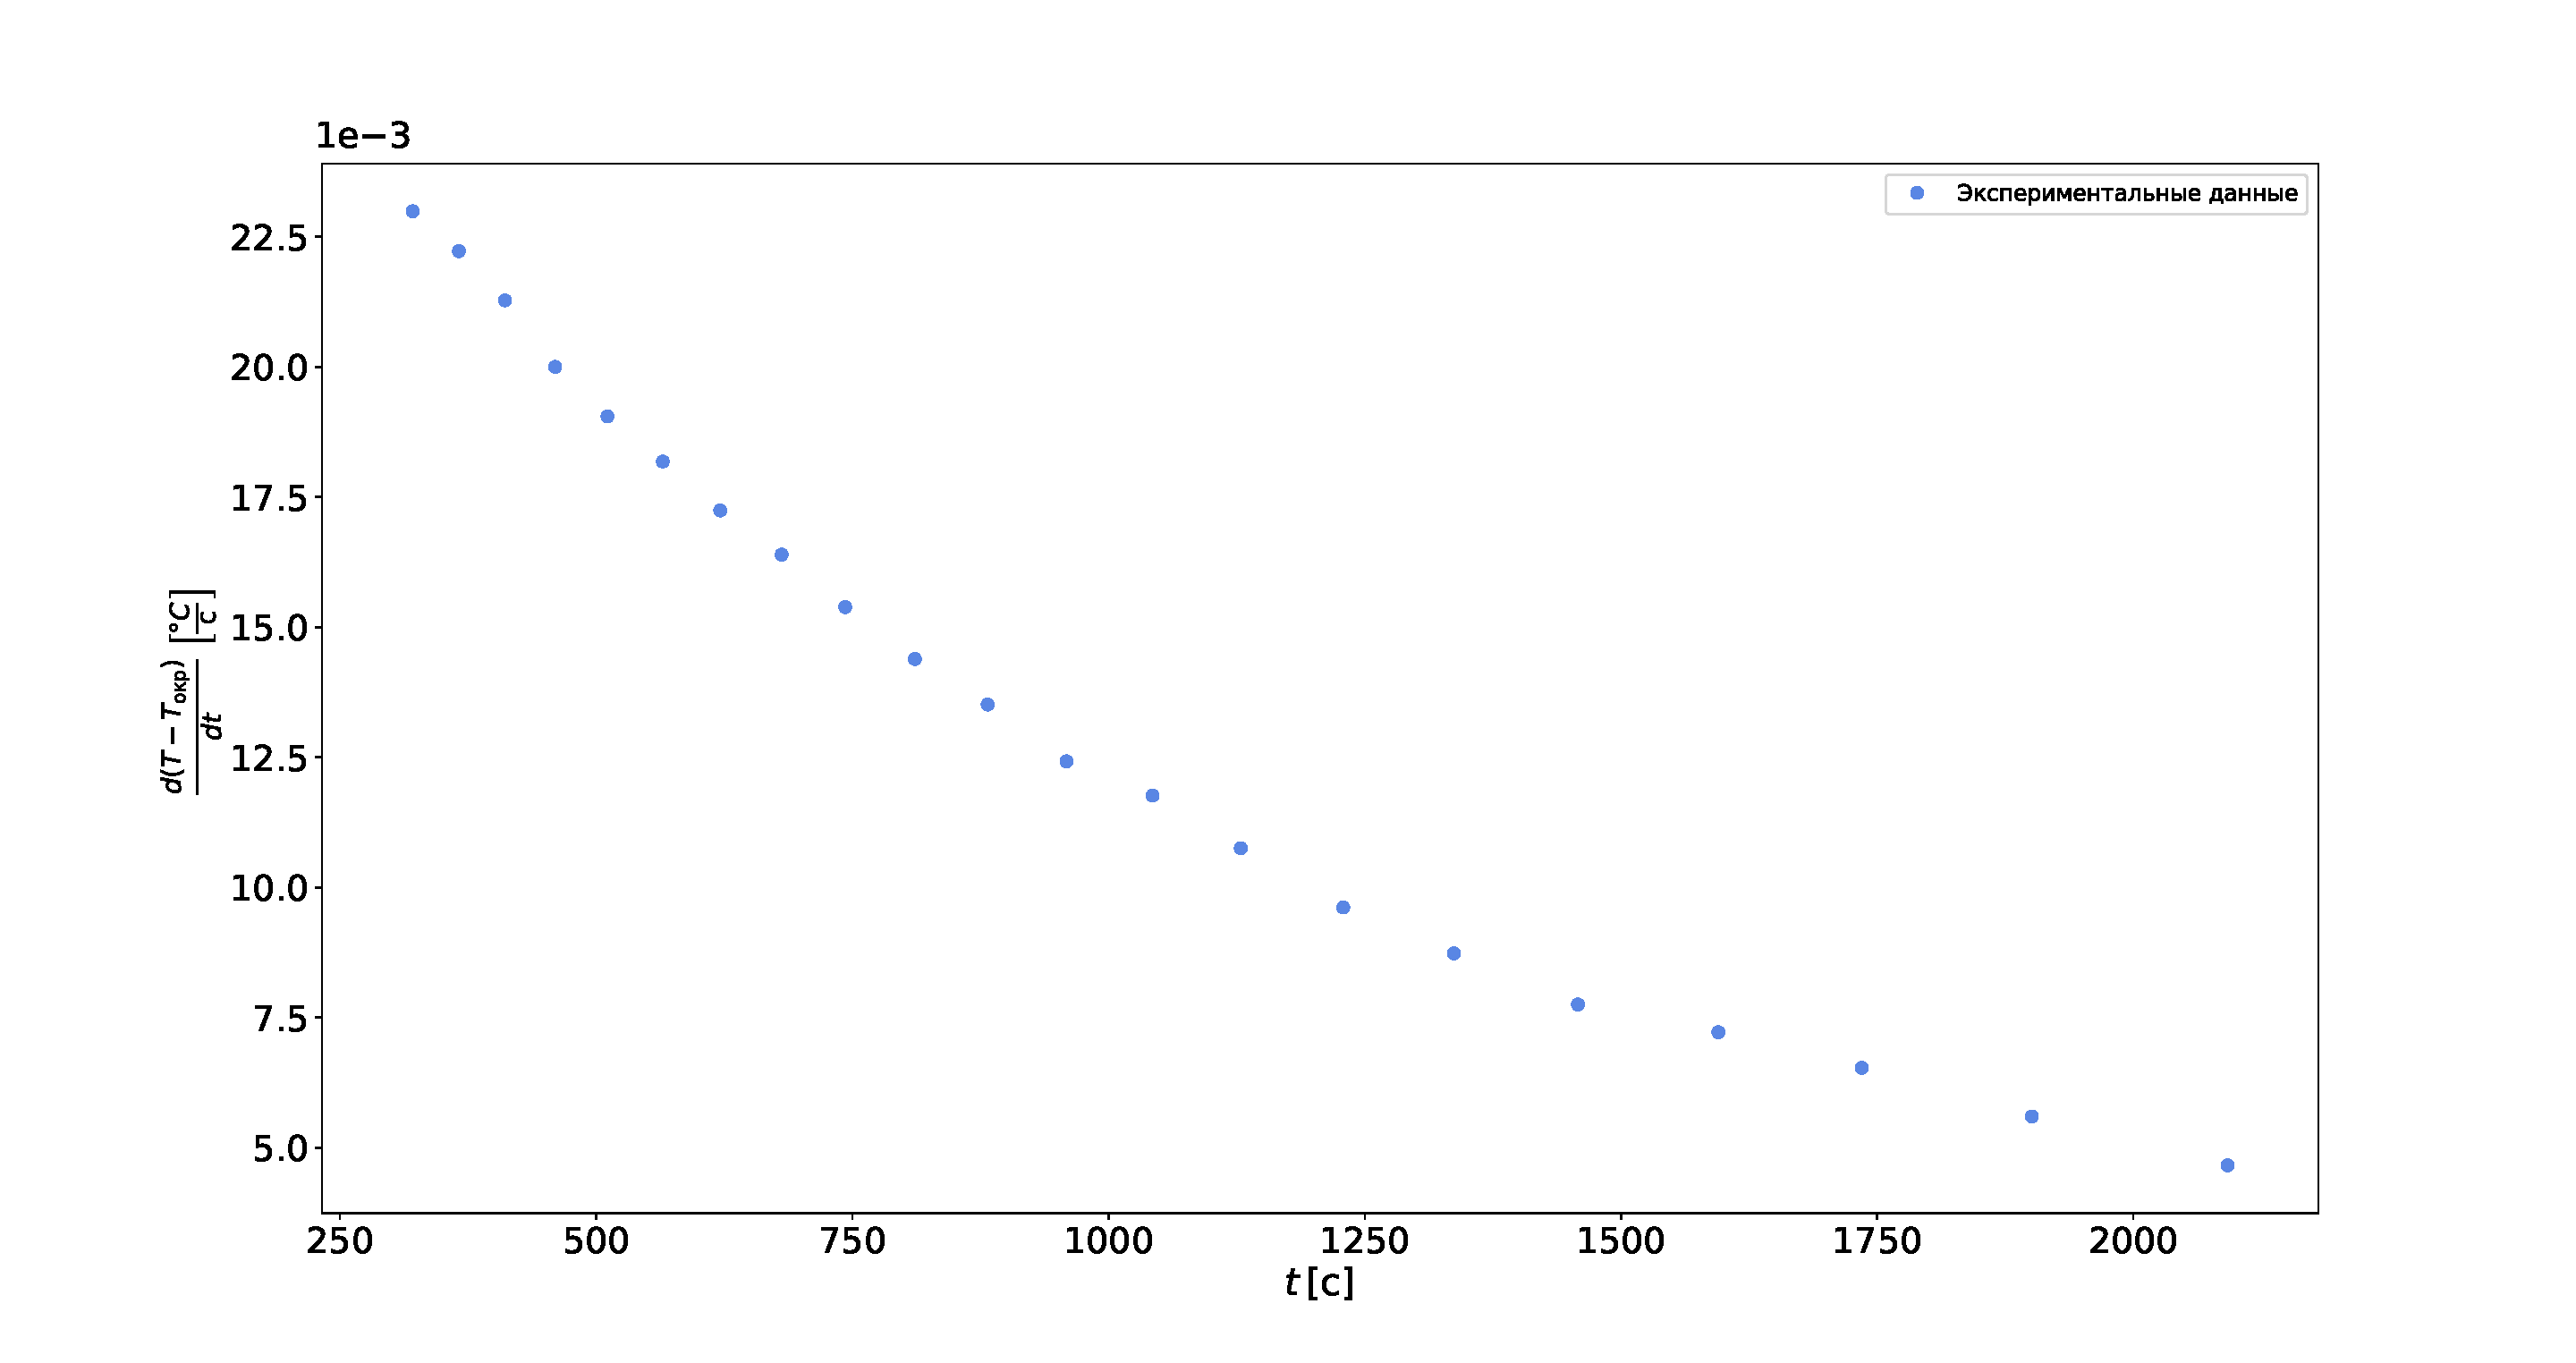
\includegraphics[width=0.55\textwidth]{gra_c.pdf}
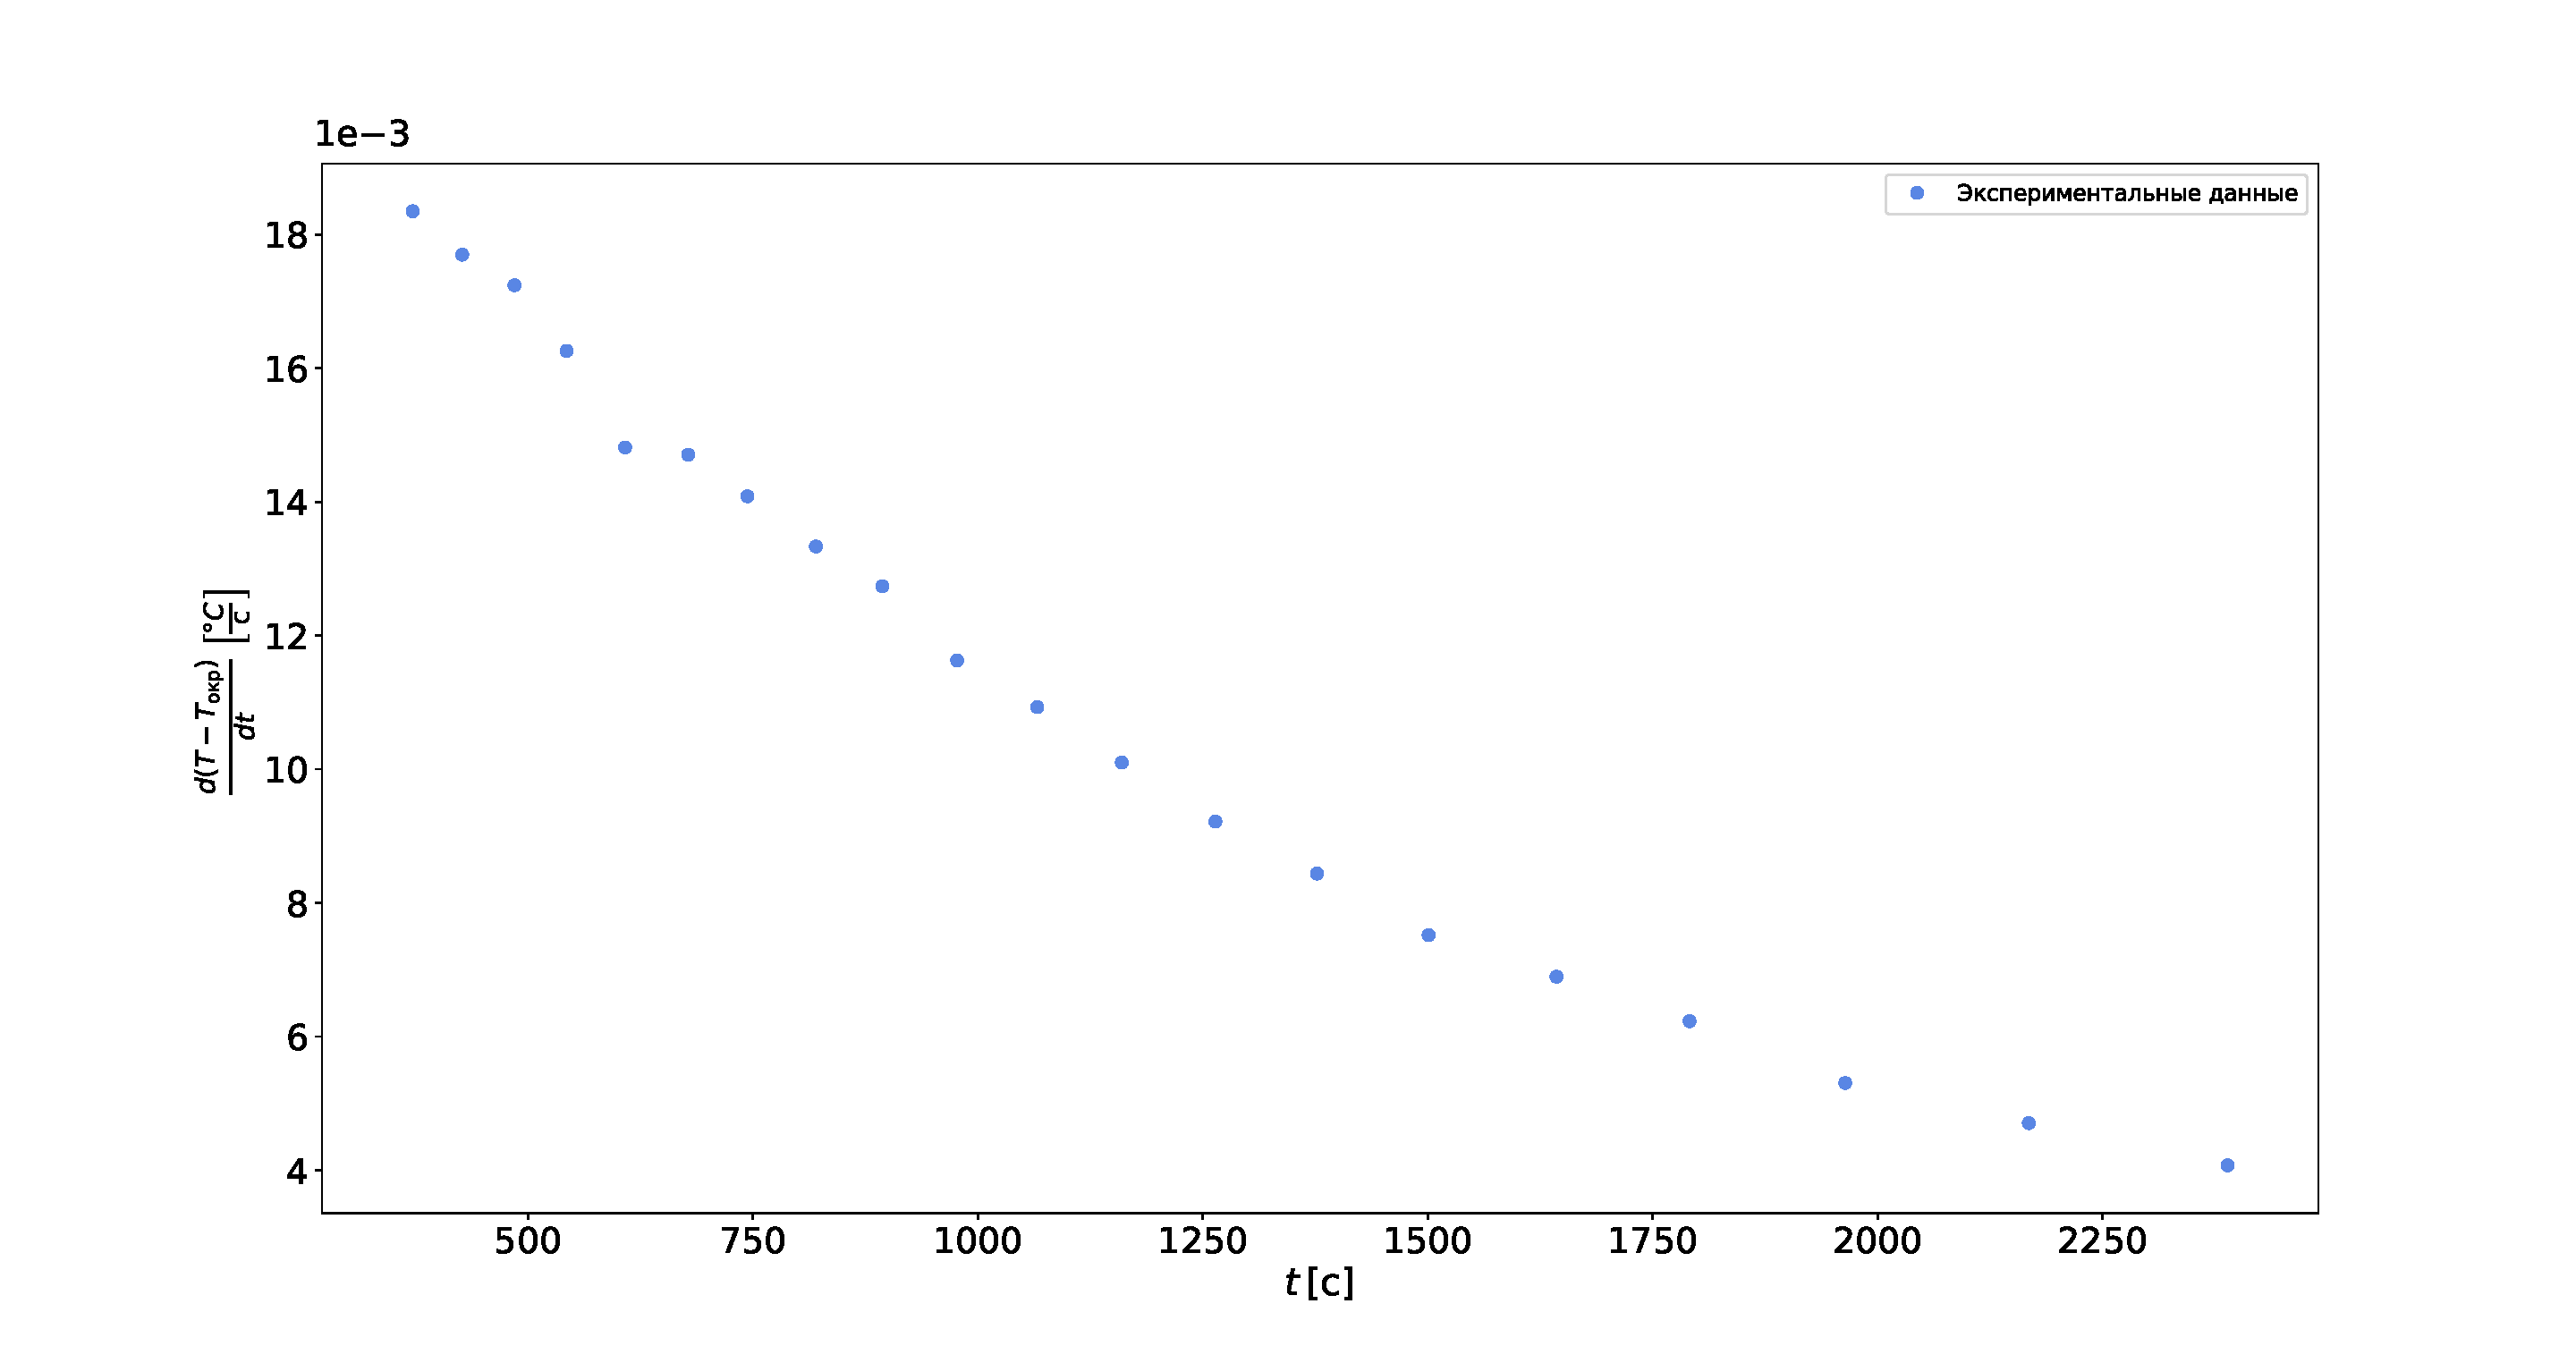
\includegraphics[width=0.55\textwidth]{gra_c_c.pdf}
\caption{Пустая камера и камера с образцом}
\end{center}
\end{figure}


Проводя аналогичные вычисления для обеих таблиц, а также логарифмируя полученные величины, получаем следующие значения:


\begin{figure}[H]
\begin{center}
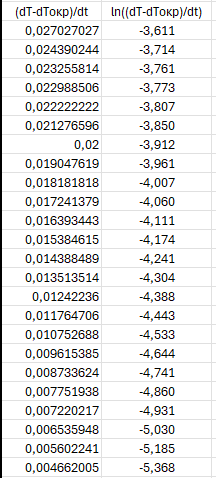
\includegraphics[width=0.2\textwidth]{3}
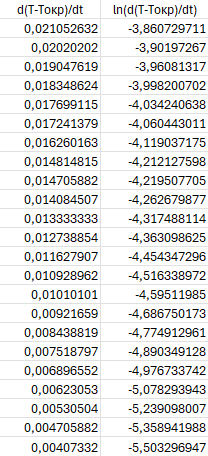
\includegraphics[width=0.2\textwidth]{4}
\caption{Пустая камера и камера с образцом}
\end{center}
\end{figure}

Так же получаем два графика:
\begin{figure}[H]
\begin{center}
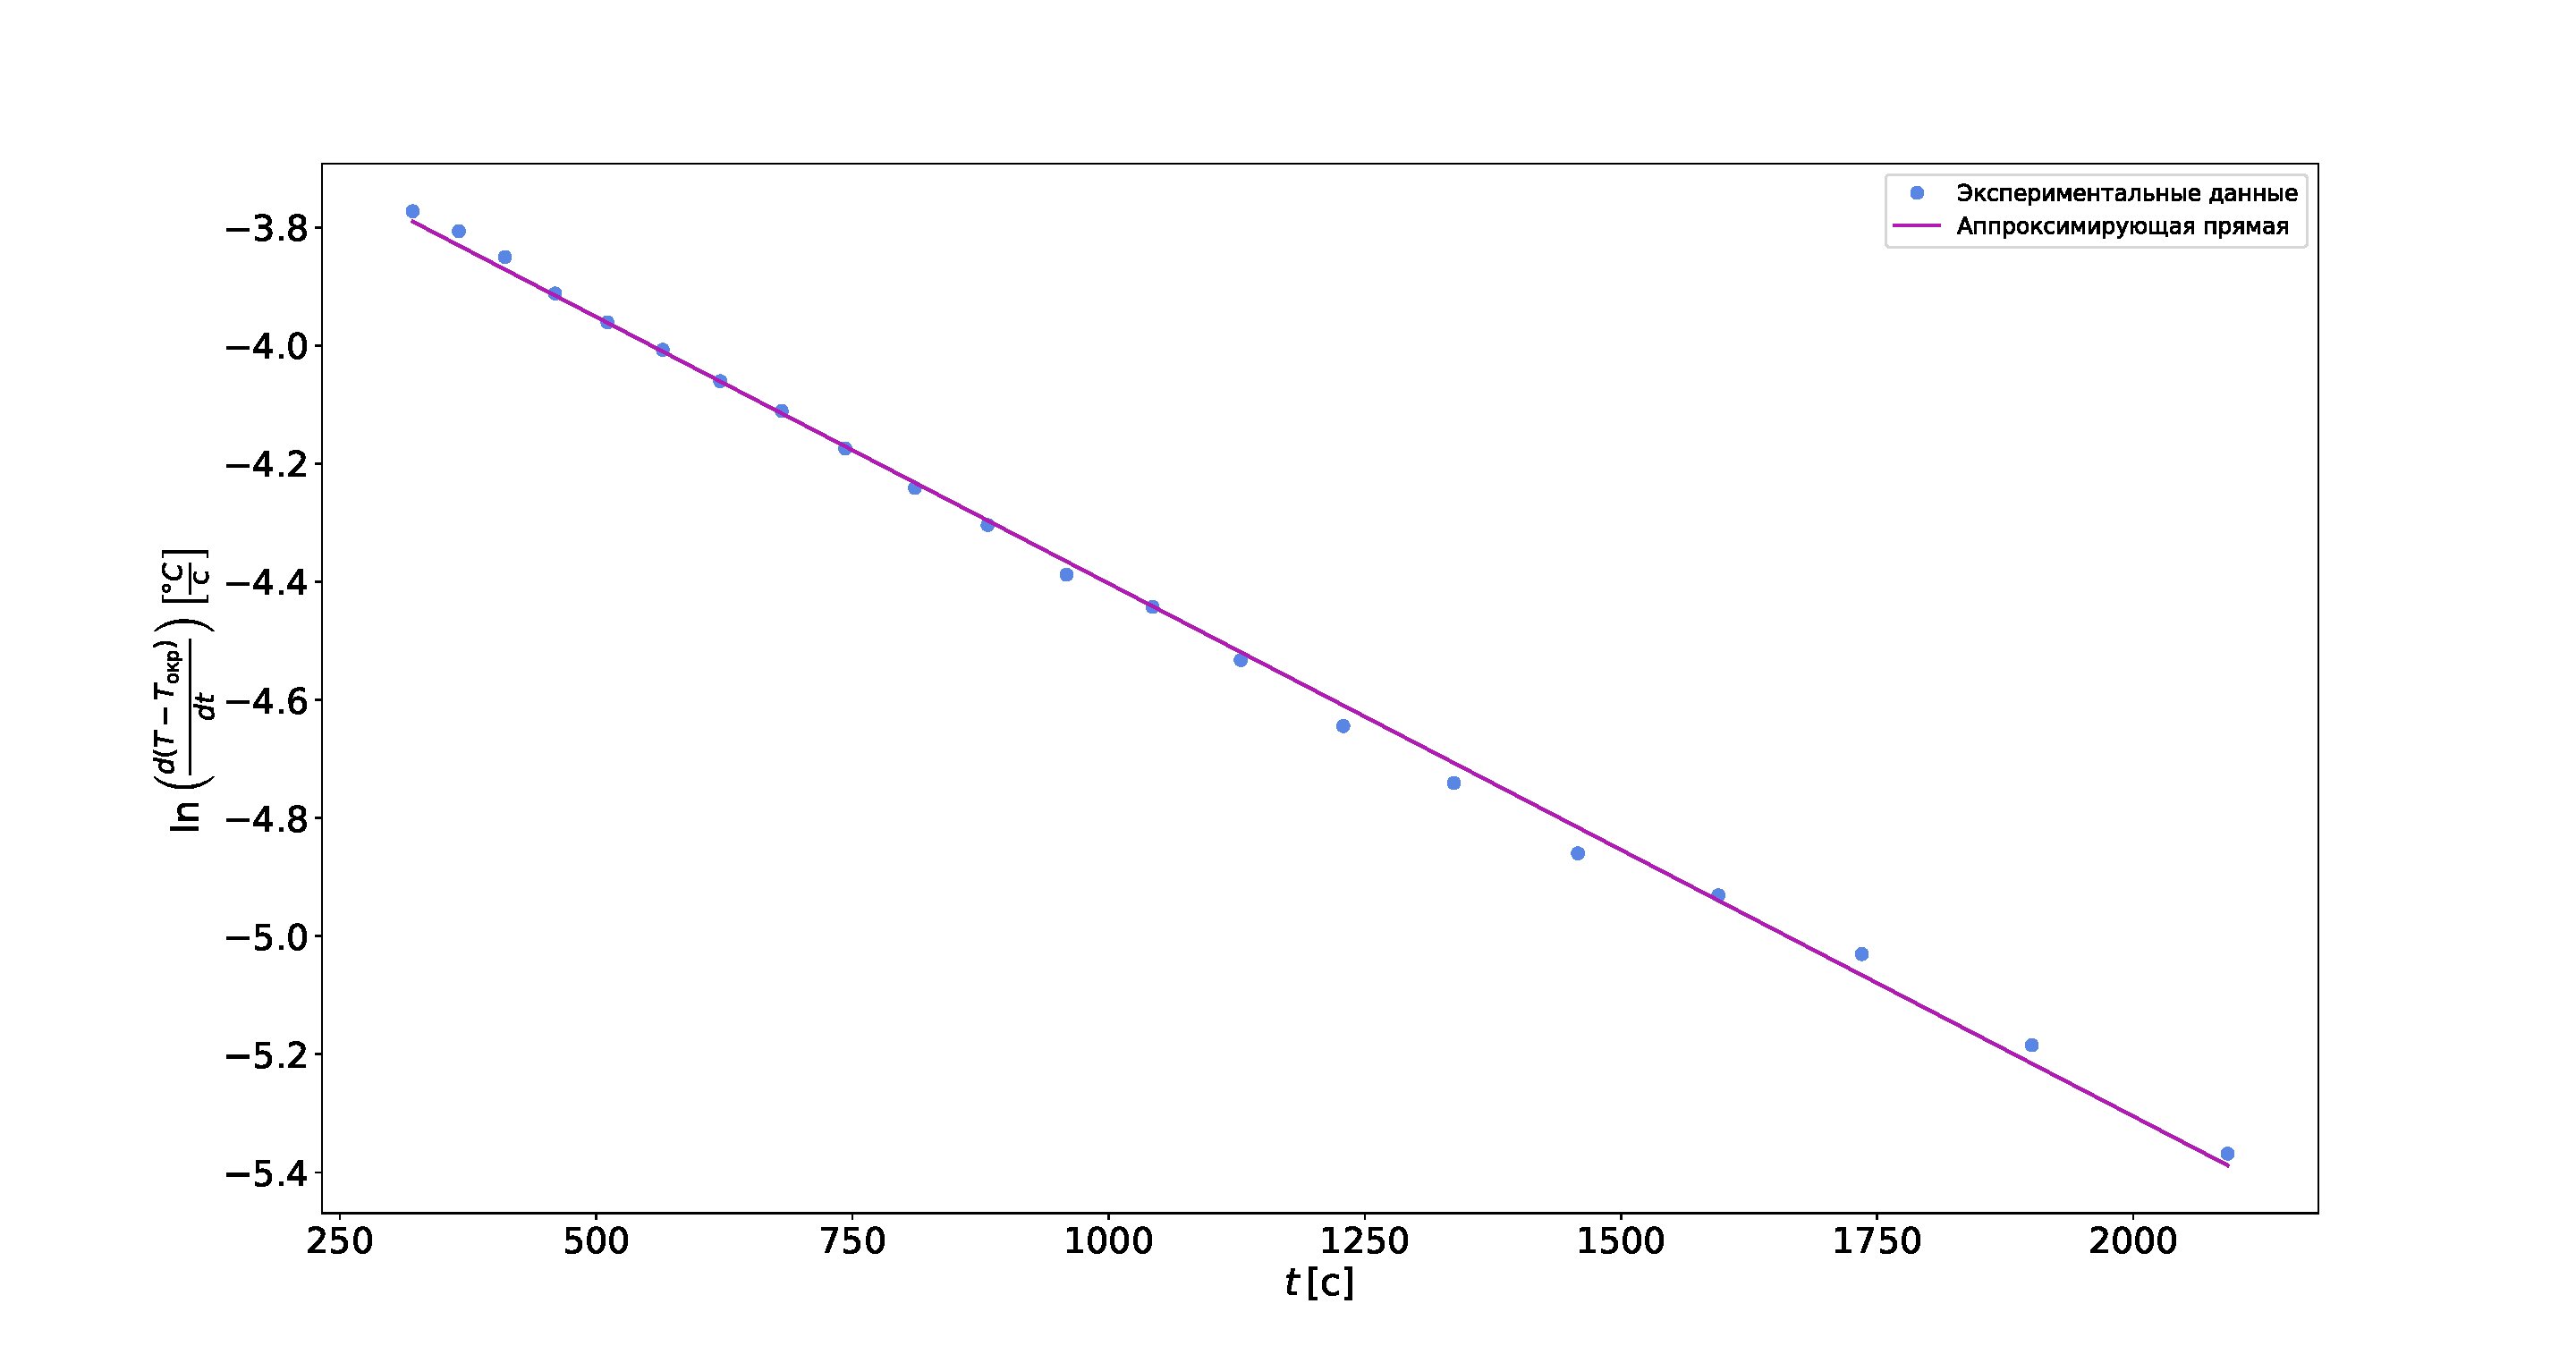
\includegraphics[width=0.55\textwidth]{gra_c_log.pdf}
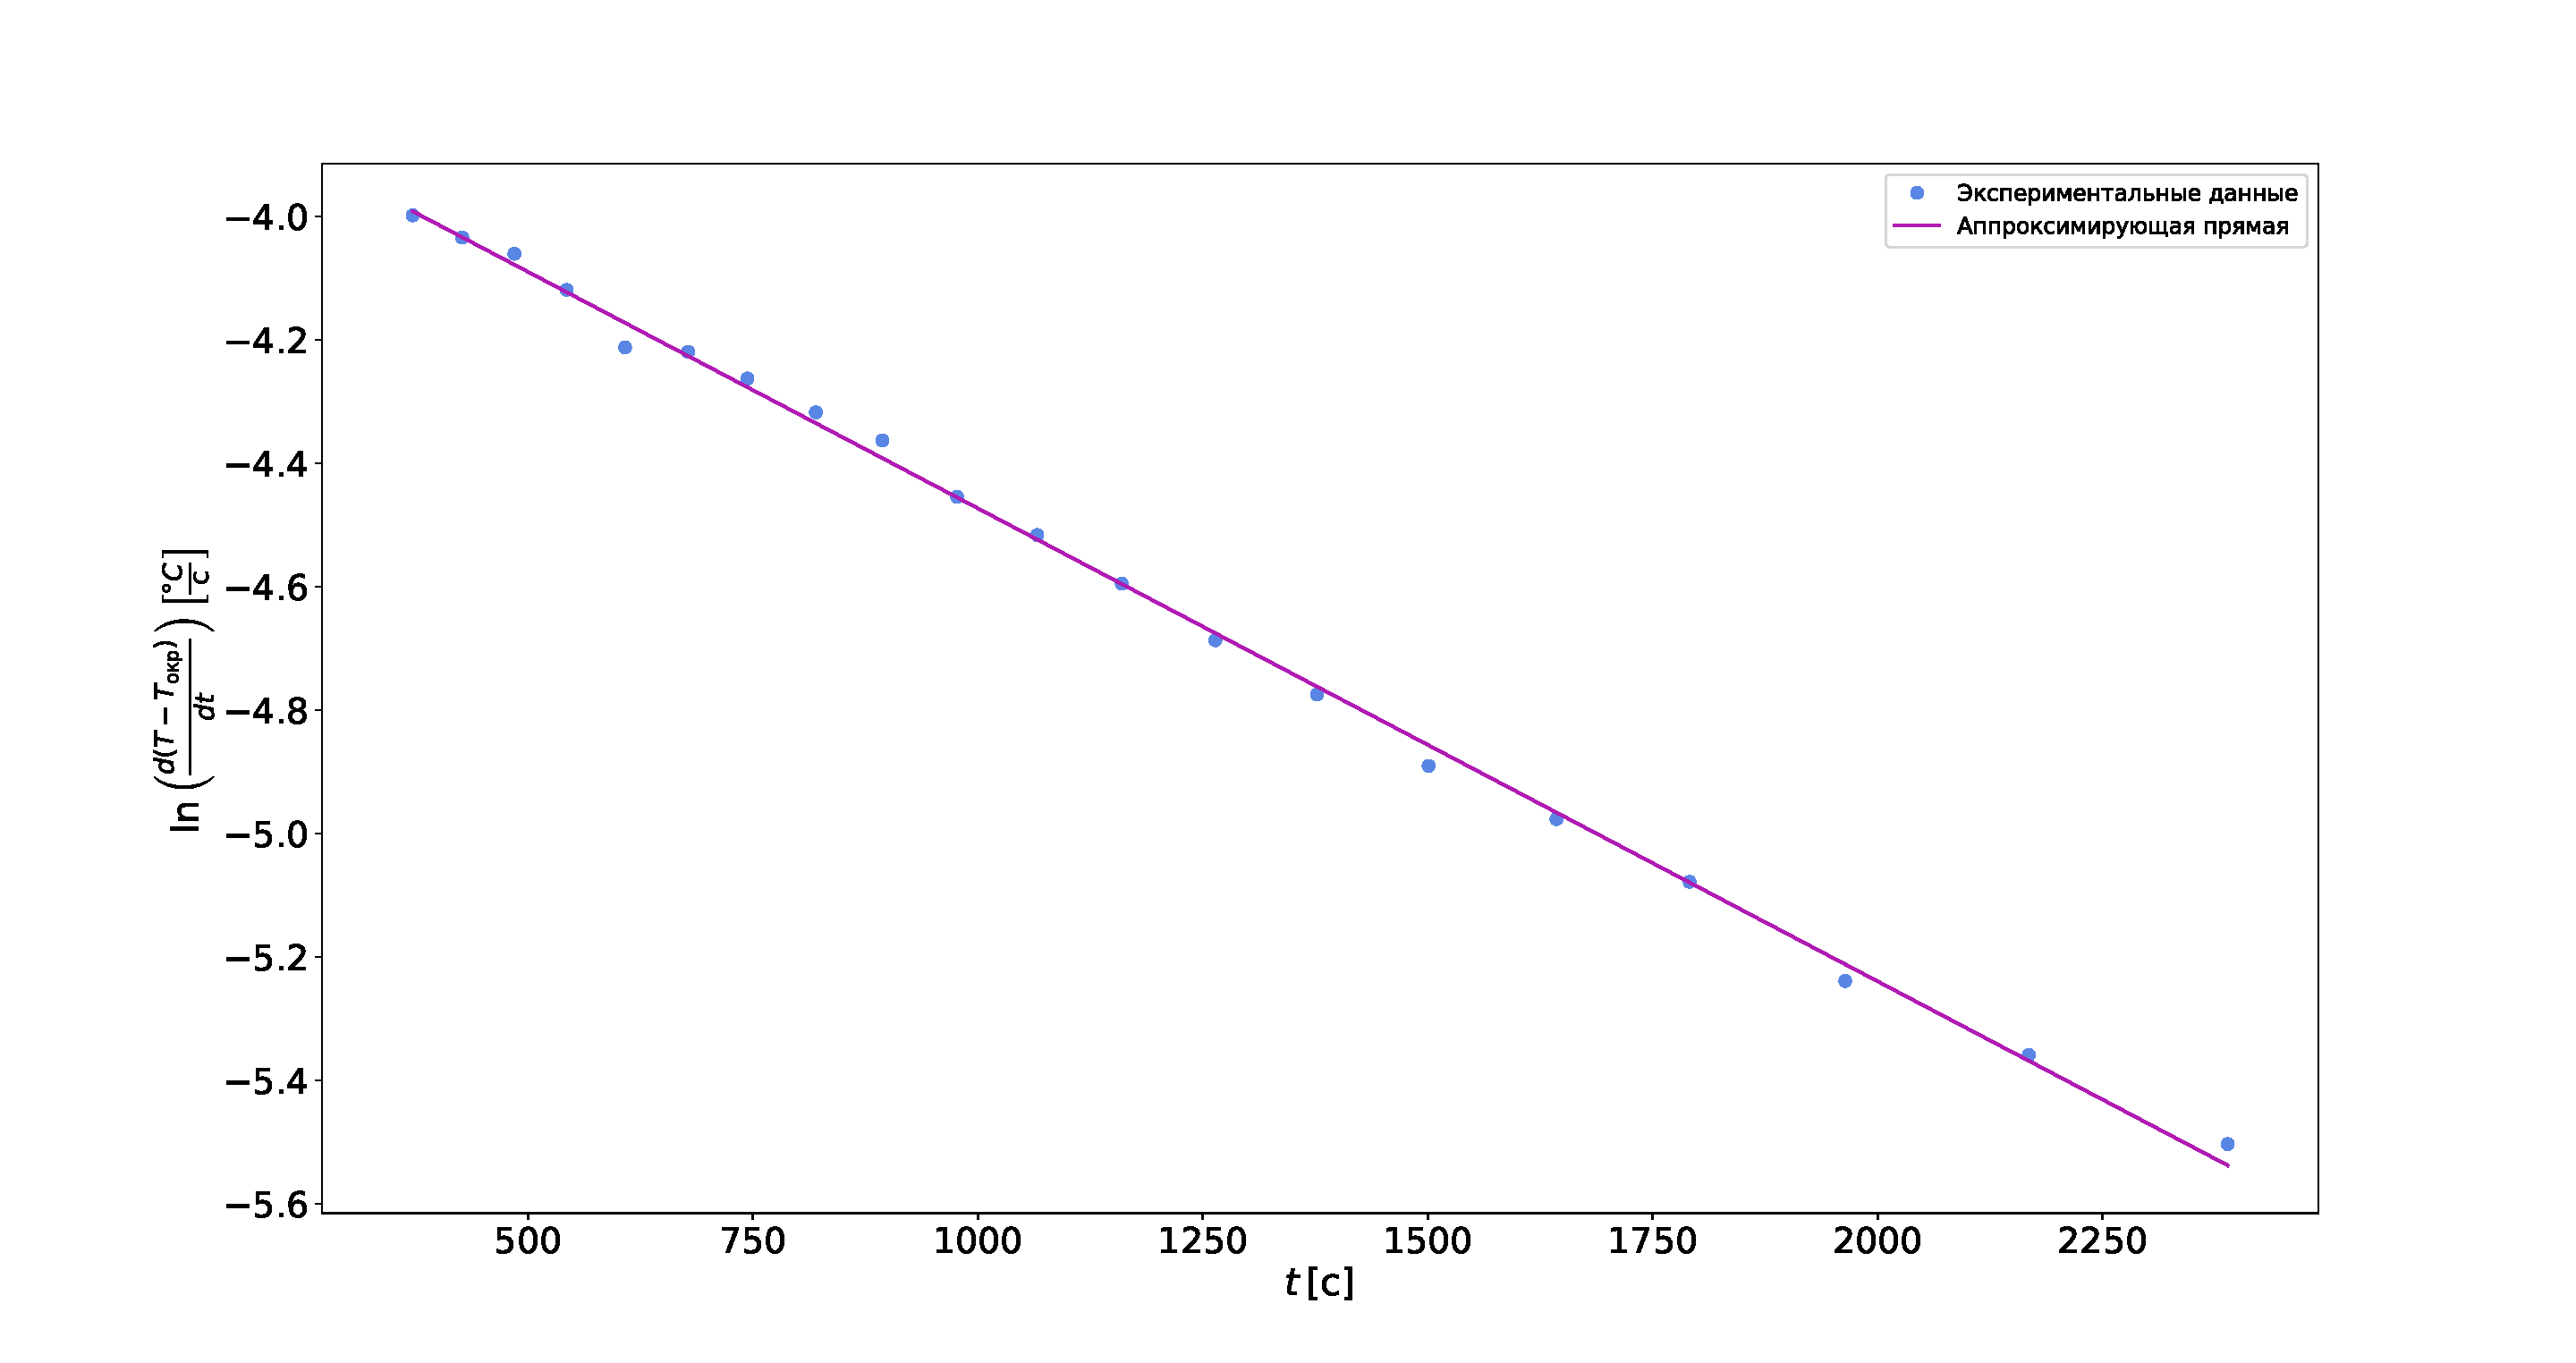
\includegraphics[width=0.55\textwidth]{gra_c_c_log.pdf}
\end{center}
\end{figure}

Найдем коэффициенты прямой по МНК. Для начала найдем $\overline{t}$ и $\overline{\ln\left(\frac{d(T-T_{окр})}{dt}\right)}$.

$\overline{t} = 886 $ c;  $\overline{\ln\left( \frac{d(T-T_{окр})}{dt} \right)} = -4.37$

Далее находим коэффициенты прямой $a$ и $b$.

$$b = \dfrac{\mathlarger{\sum}\left(t_i-\overline{t}\right)\cdot\left(\ln\left( \frac{d(T-T_{окр})}{dt}\right)_i - \overline{\ln\left( \frac{d(T-T_{окр})}{dt}\right)} \right)}{\mathlarger{\sum}\left(t_i-\overline{t}\right)^2} = -3.5$$

$$a = \overline{\ln\left(\frac{d(T-T_{окр})}{dt}\right)} -b\cdot\overline{t} = -0.0009$$\\
По аналогии находим коэффициенты прямой $a$ и $b$ для камеры с образцом:
$a=-0.00076$, $b=-3.7$

Мощность нагревателя $P = I\cdot U=7.1\cdot0.5=3.55\ \text{Вт}$

Из формулы (13) получаем выражение для $C_0$ в пустой камере:
$$C_0=P/\exp[b]\approx 117.61\pm0.05\ [\text {Дж/°C}]$$.
По аналогии из формулы (13) получаем выражения для $C_0+C$: $$C_0+C=P/\exp[b]\approx 144.51\pm 0.05\ [\text {Дж/°C}]$$
Тогда теплоемкость образца $C=26.9\ \text{Дж/°C}$, удельная теплоемкость $c=C/m\approx633\ \text{Дж/°C $\cdot$ кг}$\\

Из отношения угловых коэфициентов: $\dfrac{C_0+C}{C_0}=1.18$, из найденных $C$ и $C_0$: $\dfrac{C_0+C}{C_0}=1.24$



\section{\textbf{Вывод}}
В данной работе было проведено измерение удельной теплоемкости тела $c=633$ (у железа удельная теплоемкость примерно 600) и получена зависимость изменения скорости роста температуры от времени, на графиках видно, что если прологарифмировать эту зависимость, то получается прямая, откуда можно сделать вывод, что изначалальная зависимость - экспонента, что подтверждается теорией. Разность полученных значений для отношения теплоемкостей в случае поиска через угловые коэфициеты и через подсчет теплоемкостей лежит в пределах погрешности, а именно они отличаются примерно на 0.05, отсюда можно сделать вывод что теория соответствует эксперименту.

\end{document}
